\documentclass[a4paper, 12pt]{report}

\usepackage[T2A]{fontenc}
\usepackage[utf8]{inputenc}
\usepackage[english, russian]{babel}

\usepackage{tikz}
\usetikzlibrary{shapes, arrows, chains}

\usepackage{graphicx}
\graphicspath{{pictures/}}

\begin{document}

\tikzstyle{decision} = [diamond, draw, fill=green!20,
text width=4.5em, text badly centered, node distance=2.5cm, inner sep=0pt]
\tikzstyle{block} = [rectangle, draw, fill=blue!20,
text width=5em, text centered, rounded corners, minimum height=4em]
\tikzstyle{terminator} = [rectangle, draw, fill=red!20,
text width=5em, text centered, rounded corners, minimum height=4em]
\tikzstyle{line} = [draw, very thick, color=black!50, -latex']

\tikzstyle{io} =[trapezium,
trapezium left angle = 70,
trapezium right angle = 110, draw,
fill = yellow!30, text width=2em, text centered, minimum height=4em]

\section{Блок-схема}
\begin{tikzpicture}[scale=2, node distance = 2cm, auto]
	\node [terminator] (start) {start};
	\node [io, below of=start] (scan) {read: n};
	\node [decision, below of=scan] (decide) {n > 99};
	\node [block, below of=decide, node distance=2.5cm, right of=decide, node distance=2.5cm] (set0) {n := n div 2};		
	\node [io, below of=decide, node distance=5cm, left of=decide, node distance=2.5cm] (print) {print: n};
	\node [terminator, below of=print] (stop) {end};
	\path [line] (start) -- (scan);
	\path [line] (scan) -- (decide);
	\path [line] (decide) |- node [near start,color=black] {yes} (set0);
	\path [line] (set0) |- (decide);
	\path [line] (decide) -| node [near start,color=black] {no} (print);
	\path [line] (print) -- (stop);
	
\end{tikzpicture}

\section{Список}
\begin{itemize}
	\item элемент списка
	\item элемент списка
	\item элемент списка
	\item элемент списка
	\item элемент списка
	\item элемент списка
\end{itemize}

\section{Изображение}
	
\begin{figure}[h!]
	\centering
	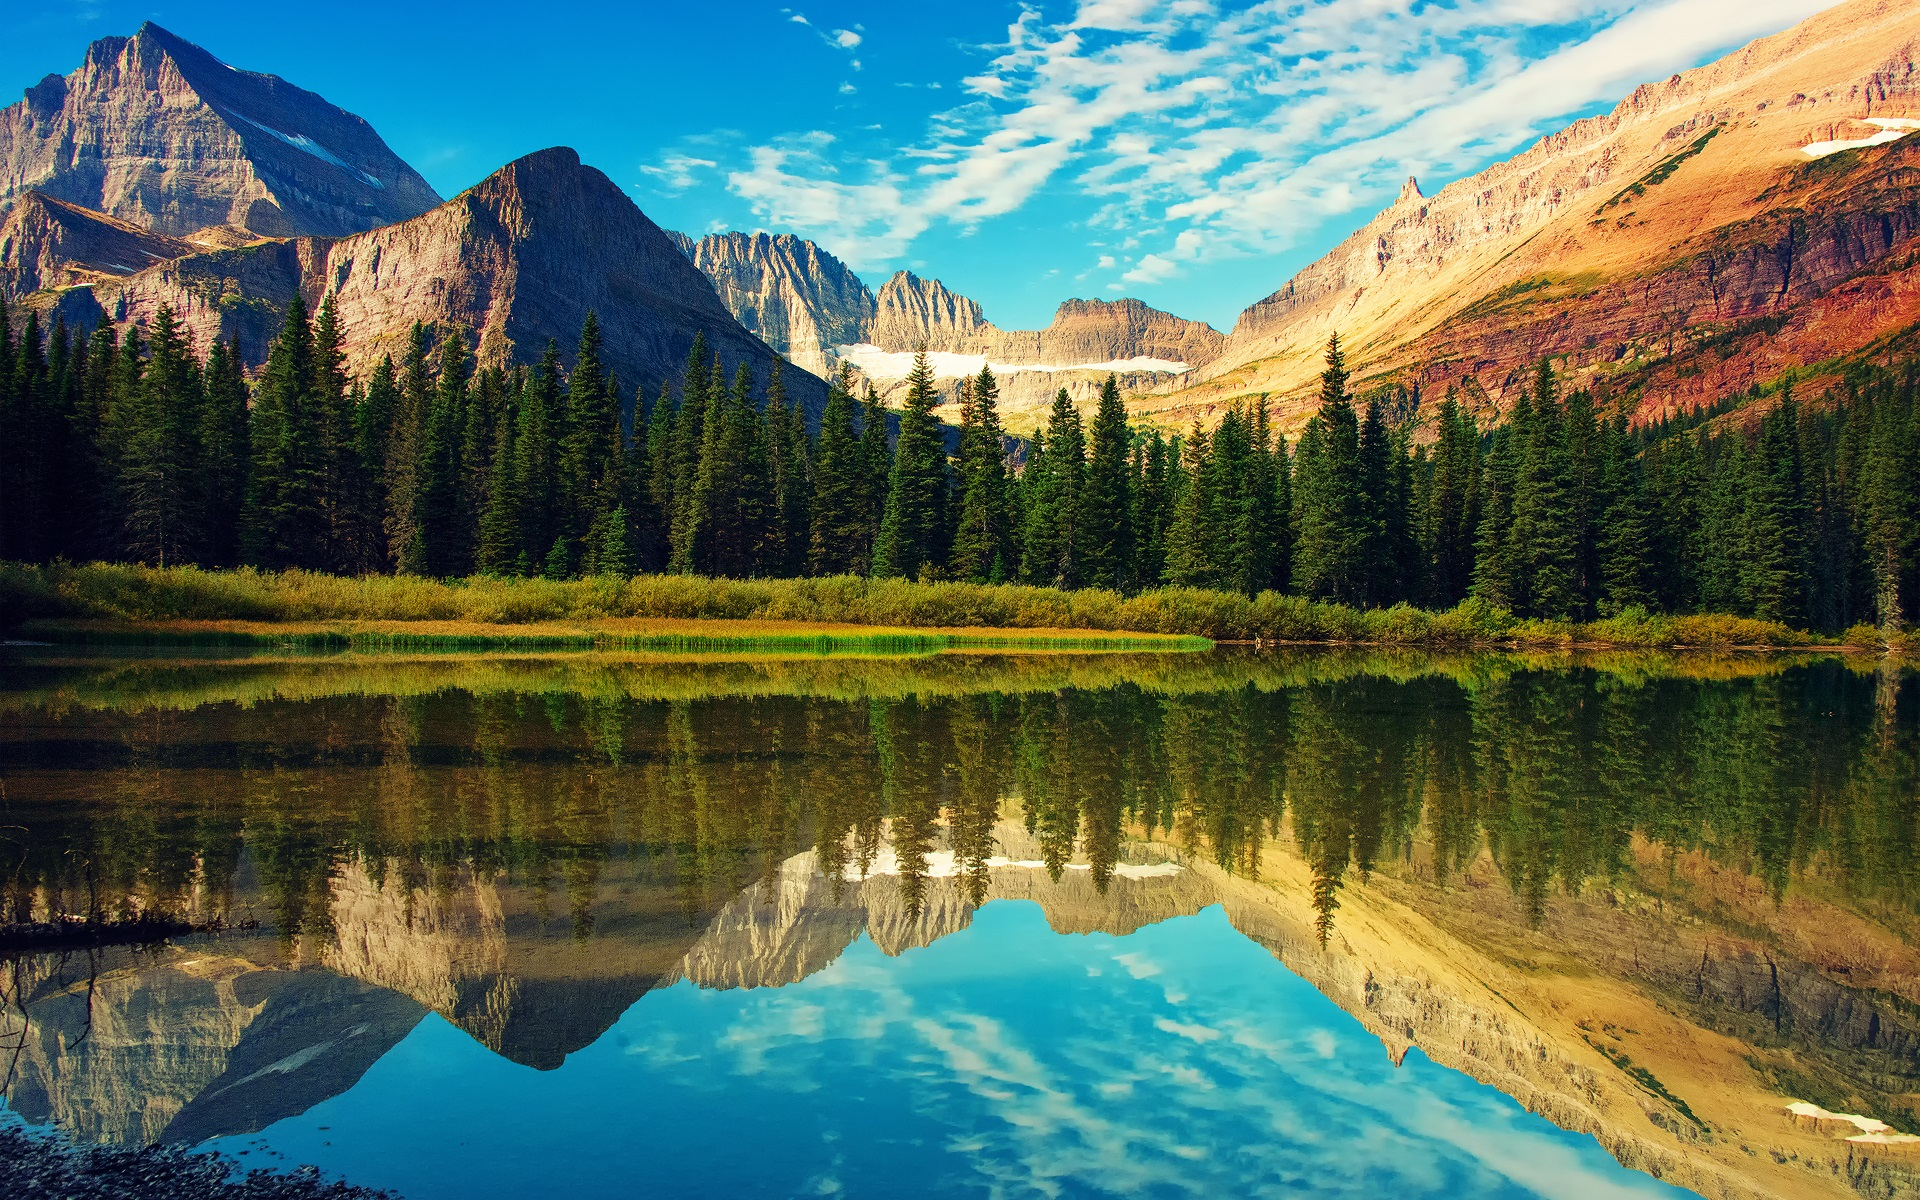
\includegraphics[width=0.7\linewidth]{NameImage.jpg}
	\caption{}
	\label{fig:-91}
\end{figure}
\end{document}
